\documentclass{article}
\usepackage[T2A]{fontenc}
\usepackage{epigraph}
\usepackage[english, russian]{babel} % языковой пакет
\usepackage{amsmath,amsfonts,amssymb} %математика
\usepackage{mathtools}
\usepackage[oglav,spisok,boldsect,eqwhole,figwhole,hyperref,hyperprint,remarks,greekit]{../../style/fn2kursstyle}
\usepackage[utf8]{inputenc}
\usepackage[]{tkz-euclide}
\usepackage{algpseudocode}
\usepackage{pgfplots}
\usepackage{tikz-3dplot}
\usepackage[oglav,spisok,boldsect,eqwhole,figwhole,hyperref,hyperprint,remarks,greekit]{./style/fn2kursstyle}
\usepackage{multirow}
\usepackage{supertabular}
\usepackage{multicol}
\usepackage{tikz}
\usepackage{pgfplots}
\usepackage{float}
\usepackage{graphicx}
\pgfplotsset{compat=1.9}
\usepackage[svgnames]{pstricks}
\usepackage{pst-solides3d} 
\usepackage{multirow}
\usepackage{hhline}
\usepackage{slashbox}
\usepackage{pdflscape}
\usepackage{array} 
\graphicspath{{../../style/}{../}}

  



\newcommand{\cond}{\mathop{\mathrm{cond}}\nolimits}
\newcommand{\rank}{\mathop{\mathrm{rank}}\nolimits}
% Переопределение команды \vec, чтобы векторы печатались полужирным курсивом
\renewcommand{\vec}[1]{\text{\mathversion{bold}${#1}$}}%{\bi{#1}}
\newcommand\thh[1]{\text{\mathversion{bold}${#1}$}}
%Переопределение команды нумерации перечней: точки заменяются на скобки
\renewcommand{\labelenumi}{\theenumi)}
\newtheorem{theorem}{Теорема}
\newtheorem{define}{Определение}
\tdplotsetmaincoords{60}{115}
\pgfplotsset{compat=newest}

\title{Решение задач интерполирования}
\author{Н.\,О.~Акиньшин}
\group{ФН2-51Б}
\date{2024}
\supervisor{А.\,С.~Джагарян}



\begin{document}
    \maketitle
    \newpage
    \tableofcontents
    \newpage

    \section{Контрольные вопросы}
    \begin{enumerate}
        \item Определите количество арифметических операций, требуемое для интерполирования функции в некоторой точке
        
        многочленом Лагранжа (включая построение самого многочлена) на сетке с числом узлов, равным $n$.
        \newline 
        {\bfseries Ответ. } 
        Запишем полином Лагранжа
        \begin{equation*}
            L_n(x) = \sum_{k=0}^{n} \prod_{j=0; j\neq k}^{n} \left(\dfrac{x-x_j}{x_k-x_j}\right) y_k 
        \end{equation*}

        Оценим количество операция для построения коэффициентов, сразу подставив 
        нужную точку. 
        \begin{equation*}
            S = (n-1) \cdot (n+1) = n^2 - 1
        \end{equation*}

        \item  Определите количество арифметических операций, требу-
        емое для интерполирования функции в некоторой точке
        
        кубическим сплайном (включая затраты на вычисление ко-
        эффициентов сплайна) на сетке с числом узлов, равным $n$.
        \newline
        {\bfseries Ответ. } Пусть имеется точка $x_0 \in [x_{i-1}, x_{i}]$, тогда по следующей формуле можно вычислить $s_i(x_0)$ за 9 операций умножения.
        \[
        s_i=a_i+b_i(x-x_{i-1})+c_i(x-x_{i-1})^2+d_i(x-x_i-1)^3, \, i=1\ldots n
        \]
        Однако для этого надо вычислить $a_i, \, b_i, \, c_i, \, d_i \, \forall i=1 \ldots n$.
        
        
        \noindent Подсчитаем количество операций требуемое для вычисления коэффициентов $a_i$. 
        \[
        a_i=y_{i-1} \, \forall i=1,2, \ldots n
        \]
        Таким образом требуется 0 операций умножения
        
        
        \noindent Подсчитаем  количество операций требуемое для вычисления коэффициентов $c_i$. Заметим, что $c_1=0$. Остальные коэффициенты можно найти решив следующую трех-диагональную систему методом прогонки. Для начало нужно вычислить следующие вспомогательные коэффициенты $h_i=x_i-x_{i-1}, \, g_i = \frac{y_i-y_{i-1}}{h_i} \,, \forall i=1 \ldots n$. Для вычисления требуется n умножений. Также 2*(n-1) для вычисления коэффициентов системы. Теперь требуется решить систему.
        \[
        h_{i-1}c_{i-1}+2(h_{i-1}+h_{i})c_i+h_i c_{i+1}=3(g_i-g_{i-1}) ,\, \forall i=1 \ldots n
        \]
        Данная система имеет размерность n-1 на n-1. Из теории известно, что для решения такой системы требуется 5*(n-1)-4 умножений.
        
        
        \noindent Подсчитаем количество операций требуемое для вычисления коэффициентов $b_i$
        \[
        b_i = g_i - \frac{(c_{i+1}+2c_i)h_i}{3}, \, \forall i=1 \ldots n
        \]
        Из формул следует, что требуется 2*n операций.
        
        
        \noindent Подсчитаем количество операций требуемое для вычисления коэффициентов $d_i$
        \[
        d_i = \frac{c_{i+1}-c_i}{3*h_i}, \, \forall i=1 \ldots n
        \]
        Из формул следует, что требуется 2*n операций.
        
        
        \noindent Итого требуется $9+n+2(n-1)+5*(n-1)-4+2n+2n=12n-2$ операций.
        \item Функция $f(x) = e^x$
        интерполируется многочленом Лагранжа на отрезке $[0, 2]$  на равномерной сетке с шагом $h = 0,2$
        Оцените ошибку экстраполяции в точке $x = 2,2$, построив многочлен Лагранжа и подставив в него это значение,
        а также по формуле для погрешности экстраполяции.
        \newline
        {\bfseries Ответ. } 
        Построим многочлен Лагранжа
        \begin{gather*}
            L_n(x) = \sum_{k=0}^{n} \prod_{j=0; j\neq k}^{n} \left(\dfrac{x-x_j}{x_k-x_j}\right) y_k = \\
            =  7.6167\cdot 10^{-7}*x^{10} + 2.53759\cdot 10^{-8}*x^9 + 3.29048\cdot 10^{-5}*x^8 + 0.000183677*x^7 + 0.00140624*x^6 + \\
            + 0.00831992*x^5 + 0.0416734*x^4 + 0.166665*x^3 + 0.5*x^2 + 1*x + 1
        \end{gather*}
        Подставим точку $x = 2.2$
        \begin{equation*}
            L_n(2.2) = 9.02501
        \end{equation*}
        Тогда погрешность
        \begin{equation*}
            |L_n(2.2) - e^{2.2}| = 3.49943*10^{-6}
        \end{equation*}
        Теперь посчитаем погрешность по формуле для экстраполяции 
        \begin{equation*}
            |f(x^*) - L_n(x^*)| \leqslant h^{n+1} \max_{y \in [a;\, b]} |f^{(n+1)(y)}|,
        \end{equation*}
        где $x^* \in [b + h, b+2h]$.
        Тогда для $x^* = 2.2$
        \begin{equation*}
            |e^{2.2} - L_n(2.2)| \leqslant 0.2^{11} e^2 \approx 1.51328*10^-7
        \end{equation*}
        \item Выпишите уравнения для параметров кубического сплай-
        на, если в узлах $x_0$ и $x_n$ помимо значений функции $y_0$ и $y_n$
        заданы первые производные $y'(x_0)$ и $y'(x_n)$
        \newline 
        {\bfseries Ответ. } 
        Сплайн на $i$-ом отрезке выглядит следующим образом $s_i=a_i+b_i(x-x_{i-1})+c_i(x-x_{i-1})^2+d_i(x-x_i-1)^3$
	Всего 4n коэффициентов. Таким образом для определения коэффициентов нужно 4n условий.
	
	
	\noindent Сплайн должен проходить через все заданные точки т.е. должно выполняться условие $S(x_i)=y_i$, что тоже самое $s_i(x_{i-1})=y_{i-1}, s_i(x_i)=y_i, \, \forall i=1 \ldots n$. Отсюда получаем 2т условий.
	
	
	\noindent Из условия непрерывности первой и второй производной (т.е. производные справа и слева в узлах сетки должны совпадать) для внутренних узлов сетки получаем.
	\[
	S'(x_i-0)=S'(x_i+0), \, S''(x_i-0)=S''(x_i+0), \, \forall i=1 \ldots n-1
	\]
	Данные условия можно переписать, как
	\[
	S'_i(x_i)=S'_{i+1}(x_i), \, S''_i(x_i)=S''_{i+1}(x_i), \, \forall i=1 \ldots n-1
	\]
	
	
	\noindent Получили 4n-2 условий требуется еще 2 условия. В классической интерполяции полагаются условия $S''(x_0)=S''(x_n)=0$. Однако, поскольку даны условия на первые производные , то имеем следующие условия $S'(x_0)=y'_0, \, S'(x_n)=y'_n$ либо, что тоже самое $S'_1(x_0)=y'_0,\, S'_n(x_n)=y'_n$
	
	
	\noindent В итоге коэффициенты $a_i, b_i,c_i,d_i$ можно найти из следующей системы
	\begin{equation}
		\centering
		\left\{\begin{split}
			S_i(x_{i-1})&=y_{i-1}, S_i(x_i)=y_i, \, \forall i=1 \ldots n \\
			S'_i(x_i)&=S'_{i+1}(x_i), \, S''_i(x_i)=S''_{i+1}(x_i), \, \forall i=1 \ldots n-1\\
			S'_1(x_0)&=y'_0,\, S'_n(x_n)=y'_n
		\end{split}\right.
	\end{equation}
	Все условия останутся такими же за исключением двух условий на краях т.е будут верны следующие формулы
	\begin{equation}
		\centering
		\left\{\begin{split}
			y_{i-1} = a_i, \, i= 1 \ldots n\\
			y_i = a_i +b_i h_i+c_ih_i^2+d_ih_i^3, \,i= 1 \ldots n\\
			b_i+2c_ih_i+3d_i h_i^2=b_{i+1}, \,i= 1 \ldots n-1\\
			2c_i+6d_ih_i=2c_{i+1}, \,i= 1 \ldots n-1\\
			b_1 = y_0' \\ 
			b_n + 2c_n h_n +3d_n h_n^2 = y_n ' 
		\end{split}\right.
	\end{equation}
        \item Каковы достоинства и недостатки сплайн-интерполяции
        и интерполяции многочленом Лагранжа?
        \newline 
        {\bfseries Ответ. } 
        \begin{enumerate}
            \item Интерполяционный полином Лагранжа имеет вид $L_n(x)=\sum_{k=0}^{n}f_k\prod_{i=0,i\neq k}^{n} \frac{x-x_i}{x_k-x_i}$. Также интерполяция Лагранжа является глобальной т.е. один полином приближает функцию, в отличии от интерполяции Сплайном, где на каждом отрезке свой приближающий полином.
	
	
            \noindent При добавлении точек многочлен Лагранжа приходиться полностью пересчитывать, в отличии от интерполяции сплайном в котором, придется либо добавить либо изменить один сплайн, а остальные сплайны не изменятся.
            
            
            \noindent Пусть значения функции f известны не точно, а лишь с некоторой погрешностью $\delta f_i: f_i= f_i^0+\delta f_i$.Как сильно исказится при этом интерполяционный полином?
            
            
            \noindent Имеем
            \[
            L_n(x) = L_n(x, f^0+\delta f) = L_n(x, f^0) + L_n(x, \delta f)
            \]
            \item Для того чтобы установить влияние погрешности входных данных на построенный полином, необходимо оценить $\max \limits_{||\delta f|| \le \delta} ||L_n(x, \delta f)||_C$
            Если ввести нормированную погрешность, то для оценки
            влияния погрешности входных данных требуется вычислить
            величину $\eta = \max \limits_{||\widetilde{\delta f})|| \le 1} ||L_n(x, \widetilde{\delta f})||_C$
            
            Для равномерной сетки $\eta=O(2^n)$. Для $\eta = O(lnn)$. Таким образом погрешности связанные с неточностью входной информации при глобальной интерполяции сильно возрастают. 
            \item  Если функция не имеет n+1 ой ограниченной производной, то погрешность в случаи глобальной интерполяции в отличии от интерполяции сплайном может вести себя плохо. Рассмотрим следующие теоремы 
	
	
            Теорема(Фабера). Для любой последовательности сеток, существует непрерывная на отрезке функция f(x) такая, что  последовательность $\{L_n(x)\}$ не сходится равномерно $f(x)$
            
            
            Теорема(Марцинкевича). Для любой непрерывной на отрезке функции f(x) существует последовательность сеток такая, что $\{L_n(x)\} \rightrightarrows f(x)$
            
            Например рассмотрим функцию $f(x) = \frac{1}{1+25x^2}$
            
            Использование глобальной полиномиальной интерполяции на
            равномерной сетке дает расходимость на участках $|x| \in (0.73;1)$ при бесконечном увеличении числа точек разбиения. Причиной этого, очевидно, является увеличение нормы производной данной функции при возрастании ее порядка.
            
            
            Однако при интерполяции сплайном имеет место следующая теорема
            
            
            Теорема. Пусть $u=f(x)\in C^4[a,b],\, f''(a)=f''(b)=0, \, M_4 = ||f^(4)||_C, \, S_3(x)$ -- сплайн третей степени. Тогда верно 
            \[
            ||f-S_3||_C \le C_1 M_4 h^4; \, ||f'-S_3'||_C \le C_2 M_4 h^3; \, ||f''-S_3''||_C \le C_3 M_4 h^2
            \]
            Отсюда следует, что для указанного класса функций не
            только $S_3$ сходится к $f$, но и ее первая и вторая производные сходятся к соответствующим производным. Функцию $S_3$ можно дифференцировать.
        \end{enumerate}
        
	
	
        \item Какие свойства полиномов Чебышева и чебышевских сеток Вам известны?
        \newline 
        {\bfseries Ответ. } 
        При интерполяции желательно, чтобы погрешность $||f-\widetilde{f}||$ была минимальна, также при увеличении числа точек интерполяции погрешность должна стремится к 0. Однако в случаи глобальной интерполяции(полиномом Лагранжа) 
	\[
	||f-\widetilde{f}||_C=||f-L_n|| \le \frac{M_{n+1}}{(n+1)!}||w||_C
	\]
	Таким образом выберем функцию $w(x) = \prod_{i=0}^{n}(x-x_i)$, так чтобы $||w||_C$ была минимальна т.е. требуется решить задачу $\min \limits_{x_0,\ldots ,x_n} \max \limits_{x\in [a,b]} |w(x)|$. Решением данной задачи является полином Чебышева.
	
	\[
	w(x)=T_{n+1}(x)=\frac{(b-a)^{n+1}}{2^{2n+1}} cos((n+1)arccos(\frac{2x-(b+a)}{b-a}))
	\]
	Таким образом узлы Чебышевской сетки имеют вид
	\[
	x_k=\frac{a+b}{2}+\frac{b-a}{2}cos(\frac{(2k+1)\pi}{2(n+1)})
	\]
	Также $||w||_C=\dfrac{1}{2^{2n+1}}(b-a)^{n+1}$. Итого для Чебышевской сетки имеем оценку погрешности
	\[
	||f-\widetilde{f}||\le \frac{M_{n+1}}{(n+1)!}\frac{(b-a)^{n+1}}{2^{2n+1}} = \epsilon_{ch}
	\]
	Сравним данную сетку с равномерной. Для равномерной сетки имеем оценку погрешности
	\[
	|f-L_n|\le \frac{M_{n+1}}{n+1}h^{n+1} = \frac{M_{n+1}}{n+1}(\frac{b-a}{n})^{n+1} = \epsilon_{R}
	\]
	Рассмотрим отношение погрешностей

	\[
	\frac{\varepsilon_{R}}{\varepsilon_{ch}} = (\frac{4}{e})^n \frac{1}{\sqrt{n}} \rightarrow \infty
	\]
	Следовательно при увеличении количества узлов интерполяции погрешность на Чебышевской сетке будет меньше чем на равномерной сетке(на любой сетке) в соответствующее число раз.
	
	
	\noindent 
	Для равномерной сетки $\eta=O(2^n)$. Для $\eta = O(lnn)$. Т.е. погрешность возникающая из неточности входных данных будет меньше на Чебышевской сетки чем на равномерной.
    \end{enumerate}    

    \newpage
    \section{Дополнительные вопросы}
    \begin{enumerate}
        \item Оценка количества операций для построение полинома Лагранжа
        \newline
        {\bfseries Ответ. } 
        Сначала посчитаем количество операций для построения одного коэффициента многочлена Лагранжа.
        \begin{equation*}
            c_k(x) = \prod_{j=0;j\neq k}^{n} \left(\dfrac{x-x_j}{x_k - x_j}\right)
        \end{equation*}
        Тогда одно умножение в скобке, и для перемножения $n$ многочленов 1 степени необходимо $2^n$ умножений. Тогда для 
        расчета кожффициента $ c_k(x)$ необходимо $S_1 = 2^{n-1} * (n-1) * (n-1)$, где 
        первый множитель $n-1$ отвечает за умножение в знаменатиле, а второй -- за деление получившегося многочлена $n-1$ степени 
        на знаменатель. 
        Согласно
        \begin{equation*}
            L_n(x) = \sum_{k=0}^{n} c_k(x)  y_k
        \end{equation*}
        $S_2 = S_1 + 1$ и итоговая сумма 
        \begin{gather*}
            S = (n+1)S_2 = (n+1)( 2^{n-1} * (n-1) * (n-1) + 1) = 1 + 2^{n-1} +\\ 
            n + 2^{n-1} n - 2^n n + 2^{n-1} n^2 - 
            2^n n^2 + 2^{n-1} n^3
        \end{gather*}
        \item Почему на функции Рунге норма ошибки стремится к бесконечности при достаточно большом количестве узлов?
        \newline
        Если рассматривать интерполяцию Лагранжа на равномерной сетке, то оценка погрешности оценивается по следующей формуле
        \[
        ||f-L_n|| \le \frac{||f^{n+1}(x)||}{n+1} \cdot (\frac{b-a}{n})^{n+1}
        \]
        При увеличении количества точек интерполяции норма ошибка растет. Это связано с тем, что $||f^(n+1)||$ не ограничено при росте $n$. Однако, только этого было бы не достаточно. Оказывается, что $||f^{(n+1)}||$ растет быстрее чем $(\frac{b-a}{n})^{n+1} \cdot \frac{1}{n}$. Для того, чтобы это показать проведем расчеты в wolfram mathematica. Рассмотрим таблицу
        \begin{table}[H]
        	\centering
        	\caption{Норма ошибки пример рунге равномерная сетка}
        	\begin{tabular}{|c|p{5cm}|p{5cm}|}
        		\hline
        		Количество узлов $n$ & Норма ошибки интерполяции
        		на равномерной сетке \\ \hline 
        		10 & < 0.4 \\ \hline 
        		40 & $10^{-6}$ \\ \hline 
        		70 & < 0.005 \\ \hline
        		100 & $10^9$ \\ \hline
        		130 & $10^{43}$ \\ \hline
        		199 & $10^{112}$\\ \hline
        	\end{tabular}
        \end{table}
        
        
        На чебышевской сетке ситуация немного улучшиться за счет того что корни распределены ближе к краям отрезка. В случаи Чебышевской сетки погрешность можно оценить по формуле
        \[
        ||f-L_n||\le \frac{M_{n+1}}{(n+1)!}\frac{(b-a)^{n+1}}{2^{2n+1}} = \epsilon_{ch}
        \]
		Проведем аналогичные расчеты для чебышевской сетки.
		
		\begin{table}[H]
			\centering
			\caption{Норма ошибки пример рунге чебышевская сетка}
			\begin{tabular}{|c|p{5cm}|p{5cm}|}
				\hline
				Количество узлов $n$ & Норма ошибки интерполяции
				на равномерной сетке \\ \hline 
				30 & < 0.35 \\ \hline 
				100 & $10^9$ \\ \hline
				130 & $10^{43}$ \\ \hline
				187 & $10^{106}$\\ \hline
			\end{tabular}
		\end{table}
		
        {\bfseries Ответ. } 
        Если рассматривать интерполяцию Лагранжа на равномерной сетке, то оценка погрешности оценивается по следующей формуле
        \[
        ||f-L_n|| \le \frac{||f^{n+1}(x)||}{n+1} \cdot (\frac{b-a}{n})^{n+1}
        \]
        При увеличении количества точек интерполяции норма ошибка растет. Это связано с тем, что $||f^(n+1)||$ не ограничено при росте $n$. Однако, только этого было бы не достаточно. Оказывается, что $||f^{(n+1)}||$ растет быстрее чем $(\frac{b-a}{n})^{n+1} \cdot \frac{1}{n}$. Для того, чтобы это показать проведем расчеты в wolfram mathematica. Рассмотрим таблицу
        \begin{table}[H]
        	\centering
        	\caption{Норма ошибки пример рунге равномерная сетка}
        	\begin{tabular}{|c|p{5cm}|p{5cm}|}
        		\hline
        		Количество узлов $n$ & Норма ошибки интерполяции
        		на равномерной сетке \\ \hline 
        		10 & < 0.4 \\ \hline 
        		40 & $10^{-6}$ \\ \hline 
        		70 & < 0.005 \\ \hline
        		100 & $10^9$ \\ \hline
        		130 & $10^{43}$ \\ \hline
        		199 & $10^{112}$\\ \hline
        	\end{tabular}
        \end{table}
        
        
        На чебышевской сетке ситуация немного улучшиться за счет того что корни распределены ближе к краям отрезка. В случаи Чебышевской сетки погрешность можно оценить по формуле
        \[
        ||f-L_n||\le \frac{M_{n+1}}{(n+1)!}\frac{(b-a)^{n+1}}{2^{2n+1}} = \epsilon_{ch}
        \]
		Проведем аналогичные расчеты для чебышевской сетки.
		
		\begin{table}[H]
			\centering
			\caption{Норма ошибки пример рунге чебышевская сетка}
			\begin{tabular}{|c|p{5cm}|p{5cm}|}
				\hline
				Количество узлов $n$ & Норма ошибки интерполяции
				на равномерной сетке \\ \hline 
				30 & < 0.35 \\ \hline 
				100 & $10^9$ \\ \hline
				130 & $10^{43}$ \\ \hline
				187 & $10^{106}$\\ \hline
			\end{tabular}
		\end{table}
        \item Что такое многочлен, наименее отклоняющийся от 0?  
             \newline
<<<<<<< HEAD
        {\bfseries Ответ. } 
        Многочлен $T_n(x)$ степени n со старшим коэффициентом 1 для которого величина $\max\limits_{x\in [-1,1]}|T_n(x)|$ является минимальной называется многочленом наименее уклоняющегося от нуля. т.е это многочлен $\min\limits_{T_n(x)} \max_{y \in [-1;\, 1]} |T_n(x)|$.
    
    \end{enumerate}
    \newpage

    \section{Дополнительные вопросы 2}
    \begin{enumerate}
        \item Какая связь между тригонометрической и полиномиальной интерполяцией?
        \newline
        {\bfseries Ответ. } 
        Запишем тригонометрический полином на равномерной сетке 
        \begin{equation*}
            Q_n = a_0 + \sum_{k=1}^{n} (a_k \cos (k \omega x) + b_k \sin (k \omega x)),
        \end{equation*}
        где $\omega = \dfrac{2 \pi}{b-a}$.
        Чебышевская сетка задается 
        \begin{equation*}
            x_k = \frac{a+b}{2} + \frac{b-a}{2} \cos (\frac{2k-1}{2n} \pi)
        \end{equation*}
        Запишем полином Лагранжа 
        \begin{equation*}
            \sum_{k=0}^{n} f_i \prod_{i=0;i\neq k}^{n} \dfrac{x-x_i}{x_k - x_i}.
        \end{equation*}
        Запишем полином Лагранжа на чебышевской сетке 
        \begin{equation*}
            \sum_{k=0}^{n} f_i \prod_{i=0;i\neq k}^{n} \dfrac{x-\frac{a+b}{2} - \frac{b-a}{2} \cos (\frac{2i-1}{2n} \pi)}{\frac{a+b}{2} + \frac{b-a}{2} \cos (\frac{2k-1}{2n} \pi) -\frac{a+b}{2} - \frac{b-a}{2} \cos (\frac{2i-1}{2n} \pi)}.
        \end{equation*}
        Сделаем замену 
        \begin{equation*}
            x = \frac{a+b}{2} + \frac{b-a}{2} \cos \varphi
        \end{equation*}
        и подставим
        \begin{equation*}
            \sum_{k=0}^{n} f_i \prod_{i=0;i\neq k}^{n} \dfrac{ \frac{b-a}{2} \cos \varphi - \frac{b-a}{2} \cos (\frac{2i-1}{2n} \pi)}{\frac{b-a}{2} \cos (\frac{2k-1}{2n} \pi)  - \frac{b-a}{2} \cos (\frac{2i-1}{2n} \pi)}.
        \end{equation*}
        Получили произведение косинусов. Заметим, что косинус в произвольной степени легко привести к линейной комбинации $\sin$ и $\cos$. То есть получили тригонометрический полином на равномерной сетке.
        \item Есть ли смысл в чебышевской сетке при сплайн-интерполяции?
        \newline
        {\bfseries Ответ. } 
        Нет смысла, потому что для сплайн-интерполяции справедлива следующая оценка
        \begin{equation*}
            \|f - S_3\|_C \leqslant C_1 M_4 h^4
        \end{equation*}
        Для чебышевской сетки известно, что при увеличении количества точек $h \to 0$
        \item Основные отличия интерполирования при помощи полиномов Лагранжа и интерполирования при помощи сплайнов?
        \newline
        {\bfseries Ответ. } 
        \begin{enumerate}
            \item Сплайн - локальная интерполяция, полином Лагранжа - глобальная интерполяция
            \item Лагранж сильнее чувствителен к погрешностям
            \item  Если функция не имеет n+1 ой ограниченной производной, то погрешность в случае глобальной интерполяции в отличии от интерполяции сплайном может вести себя плохо.
        \end{enumerate}
    \end{enumerate}

\section{Результаты}
=======
        {\bfseries Ответ.} 
        Многочлен $T_n(x)$ степени n со старшим коэффициентом 1 для которого величина $\max\limits_{x\in [-1,1]}|T_n(x)|$ является минимальной называется многочленом наименее уклоняющегося от нуля. т.е это многочлен $\min\limits_{T_n(x)} \max_{y \in [-1;\, 1]} |T_n(x)|$.
    \end{enumerate}
    \newpage

	\item Вопрос 4. Проведите интерполирование функций f(x) = x, g(x) = $x^2$
	с помощью сплайн-интерполяции. Будет ли сплайн тождественно совпадать с функциями на f и g на отрезке [−1, 1]? Если да, то почему? Если нет, то почему?
	
	
	{\bfseries Ответ.} 
	Тождественно совпадать ни та, ни другая функция не будут это хорошо видно если взять 2 точки. Это происходит , потому что истинной зависимости мы не знаем а пытаемся восстановить функцию лишь по ее значениям в точках кубическим многочленом. Кубический многочлен с ненулевыми коэффициентами не может тожедствено приблизить линейную или квадратичную зависимость. Однако если рассмотреть аналогичный алгоритм который на каждом под отрезке строил не кубический полином а в 1ом случае линейную функцию а во 2ом квадратичный полином, то зависимости могли бы быть тождественно приближены.
    \section{Результаты}
>>>>>>> 7cdee46c01cf605ac895434ec51f6a4b4065ba36

    
    \begin{table}[H]
        \centering
        \caption{Норма ошибка в зависимости от сетки и узлов на ней для $y = x^2$}
        \begin{tabular}{|c|p{5cm}|p{5cm}|}
            \hline
            Количество узлов $n$ & Норма ошибки интерполяции
            на равномерной сетке & Норма ошибки интерполяции
            на чебышевской сетке \\
            \hline 
            4 & 1.39e-17 & 1.11e-15 \\ \hline
            8 & 1.57e-14 & 8.27e-14\\ \hline
            16 &4.16e-11 & 4.12e-10\\ \hline
            32 & 0.0013 &  0.027\\ \hline
            64 &1.8e+11 & 9.44e+13\\ \hline
            128 &3.30e+41&   3.37e+46\\ \hline
        \end{tabular}
    \end{table}
    \begin{table}[H]
        \centering
        \caption{Норма ошибка в зависимости от сетки и узлов на ней для примера Рунге}
        \begin{tabular}{|c|p{5cm}|p{5cm}|}
            \hline
            Количество узлов $n$ & Норма ошибки интерполяции
            на равномерной сетке & Норма ошибки интерполяции
            на чебышевской сетке \\
            \hline 
            4 & 0.02 &   0.01 \\ \hline
            8 & 0.002 & 0.0004\\ \hline
            16 &3.99e-05 & 3.11e-07\\ \hline
            32 &  0.003 &  0.024\\ \hline
            64 &1.33e+13 & 1.04e+14\\ \hline
            128 & 4.18e+43&   4.16e+46\\ \hline
        \end{tabular}
    \end{table}
    \begin{table}[H]
        \centering
        \caption{Норма ошибка в зависимости от сетки и узлов на ней для $y = \dfrac{1}{\arctg (1+10x^2)}$}
        \begin{tabular}{|c|p{5cm}|p{5cm}|}
            \hline
            Количество узлов $n$ & Норма ошибки интерполяции
            на равномерной сетке & Норма ошибки интерполяции
            на чебышевской сетке \\
            \hline 
            4 & 0.41 &  0.43 \\ \hline
            8 &  1.24 & 0.31\\ \hline
            16 &54.22 & 0.14\\ \hline
            32 & 194965 & 0.027\\ \hline
            64 &3.17e+16 &  5.28e+14\\ \hline
            128 &  3.24e+50&  5.39e+46\\ \hline
        \end{tabular}
    \end{table}

    \begin{table}[H]
        \centering
        \caption{Норма ошибка в зависимости от сетки и узлов на ней для $y = (4x^3 + 2x^2 - 4x + 2 )^{\sqrt{2}} + \arcsin{\dfrac{1}{5+x - x^2}} - 5$}
        \begin{tabular}{|c|p{5cm}|p{5cm}|}
            \hline
            Количество узлов $n$ & Норма ошибки интерполяции
            на равномерной сетке & Норма ошибки интерполяции
            на чебышевской сетке \\
            \hline 
            4 &  0.6 &  0.33 \\ \hline
            8 &  0.02 & 0.008\\ \hline
            16 &0.009 & 7.25e-05\\ \hline
            32 & 0.008 & 0.004\\ \hline
            64 & 6.8e+11 & 4.36e+14\\ \hline
            128 & 5.66e+43&  2.3e+47\\ \hline
        \end{tabular}
    \end{table}
    \begin{table}[H]
        \centering
        \caption{Норма ошибка в зависимости от сетки и узлов на ней для тестового примера варианта №2}
        \begin{tabular}{|c|p{5cm}|p{5cm}|}
            \hline
            Количество узлов $n$ & Норма ошибки интерполяции
            на равномерной сетке & Норма ошибки интерполяции
            на чебышевской сетке \\
            \hline 
            4 & 2.47 &  1.81 \\ \hline
            8 & 2.79 & 2.42\\ \hline
            16 &32.12 & 2.62\\ \hline
            32 & 2563.75 & 2.43\\ \hline
            64 &1.25e+13 & 2.47e+14\\ \hline
            128 & 2.99e+43&  8.25e+45\\ \hline
        \end{tabular}
    \end{table}
<<<<<<< HEAD
    \begin{table}[H]
        \centering
        \caption{Исследование скорости сходимости функции $y = \sin(\pi x)$, $h = 1$, $q = 1/3$}
        \begin{tabular}{|c|p{3cm}|p{3cm}|p{3cm}|p{3cm}|}
            \hline
            $n$ & Шаг сетки & Норма ошибки $err_n$ & Отношение ошибок $z_n = \dfrac{err_n}{err_{n-1}}$ & Порядок сходимости $p_n = \log_q z_n$ \\
            \hline 
            $1$ & $h$ & 1 & --- & --- \\
            \hline 
            $2$ & $qh$ &0.018 & 0.018 & 3.62\\
            \hline 
            $3$ & $q^2 h$ &7.45e-09 & 4.14e-7& 13.2\\
            \hline 
            $4$ & $q^3 h$ &  4.32e+09&5.79e17 &-36.8 \\
            \hline
            $5$ & $q^4 h$ &  6.75e+66&1.56e57 & -118.7\\
            \hline 
        \end{tabular}
    \end{table}


    \begin{table}[H]
        \centering
        \caption{Исследование скорости сходимости функции $y = \sin(\pi x)$, $h = 0.5$, $q = 0.5$ для сплайн-интерполяции}
        \begin{tabular}{|c|p{3cm}|p{3cm}|p{3cm}|p{3cm}|}
            \hline
            $n$ & Шаг сетки & Норма ошибки $err_n$ & Отношение ошибок $z_n = \dfrac{err_n}{err_{n-1}}$ & Порядок сходимости $p_n = \log_q z_n$ \\
            \hline 
            $1$ & $h$ & 1.39461 & --- & --- \\
            \hline 
            $2$ & $qh$ &0.764926 & 0.548487 & 0.86647\\
            \hline 
            $3$ & $q^2 h$ & 0.390168& 0.510073& 0.971225\\
            \hline 
            $4$ & $q^3 h$ &  0.196034&0.502435 &0.992992\\
            \hline 
            $5$ & $q^4 h$ &  0.0981353&0.500603 & 0.99826\\
            \hline 
        \end{tabular}
    \end{table}

    \begin{table}[H]
        \centering
        \caption{Исследование скорости сходимости функции $y = \sin(\pi x)$}
        \begin{tabular}{|c|p{3cm}|p{3cm}|p{3cm}|p{3cm}|}
            \hline
            Количество узлов $n$ & Порядок сходимости полинома Лагранжа на равномерной сетке 
            & Порядок сходимости полинома Лагранжа на чебышевской сетке 
            & Порядок сходимости сплайна на отрезке [-1, 1]
            & Порядок сходимости сплайна на отрезке [-1.25, 1.25] \\
            \hline 
            8 & ---& --- & ---& ---\\
            \hline 
            16 &20.45 & 21.76 & 0.971225& 0.411548\\
            \hline 
            32 & -22.02& -26.25 &0.992992 & 0\\
            \hline 
            64 &-48.37 & -53&0.99826 & 0\\
            \hline 
            128 &-102.515 & -105&0.999563 & 0\\
            \hline
        \end{tabular}
    \end{table}
    \begin{figure}[H]
        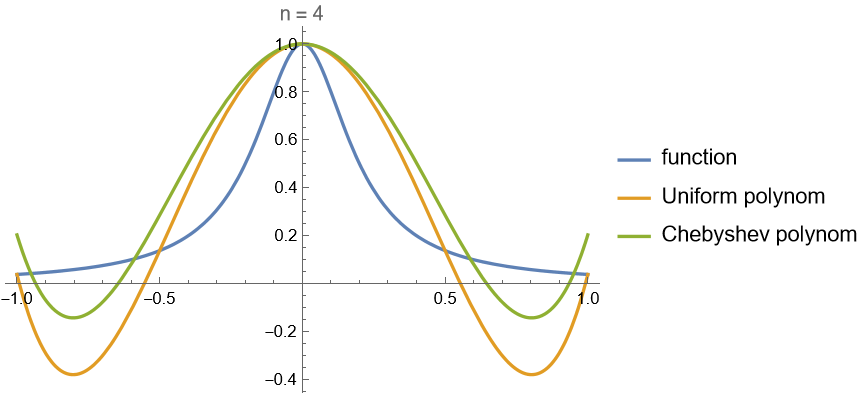
\includegraphics[width=\textwidth]{runge4.png}
        \caption{Интерполирование примера Рунге для 4 узлов многочленом Лагранжа}
    \end{figure}
    \begin{figure}[H]
        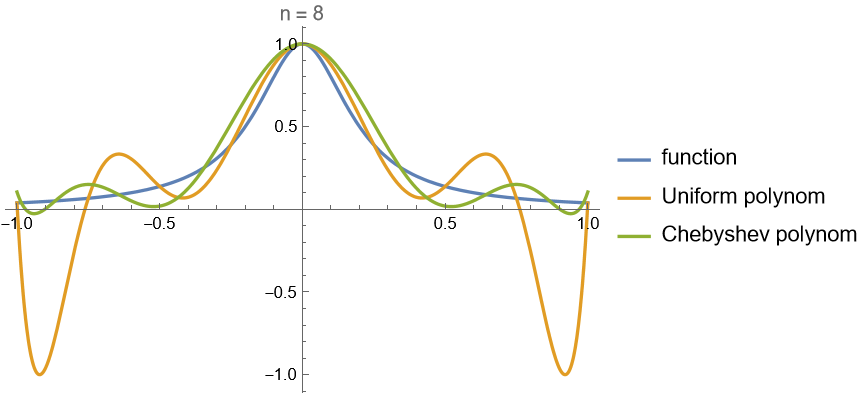
\includegraphics[width=\textwidth]{runge8.png}
        \caption{Интерполирование примера Рунге для 8 узлов многочленом Лагранжа}
    \end{figure}
    \begin{figure}[H]
        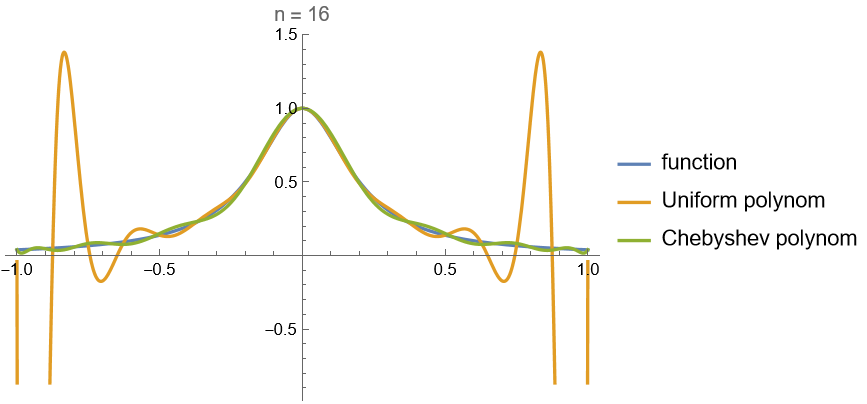
\includegraphics[width=\textwidth]{runge16.png}
        \caption{Интерполирование примера Рунге для 16 узлов многочленом Лагранжа}
    \end{figure}
    \begin{figure}[H]
        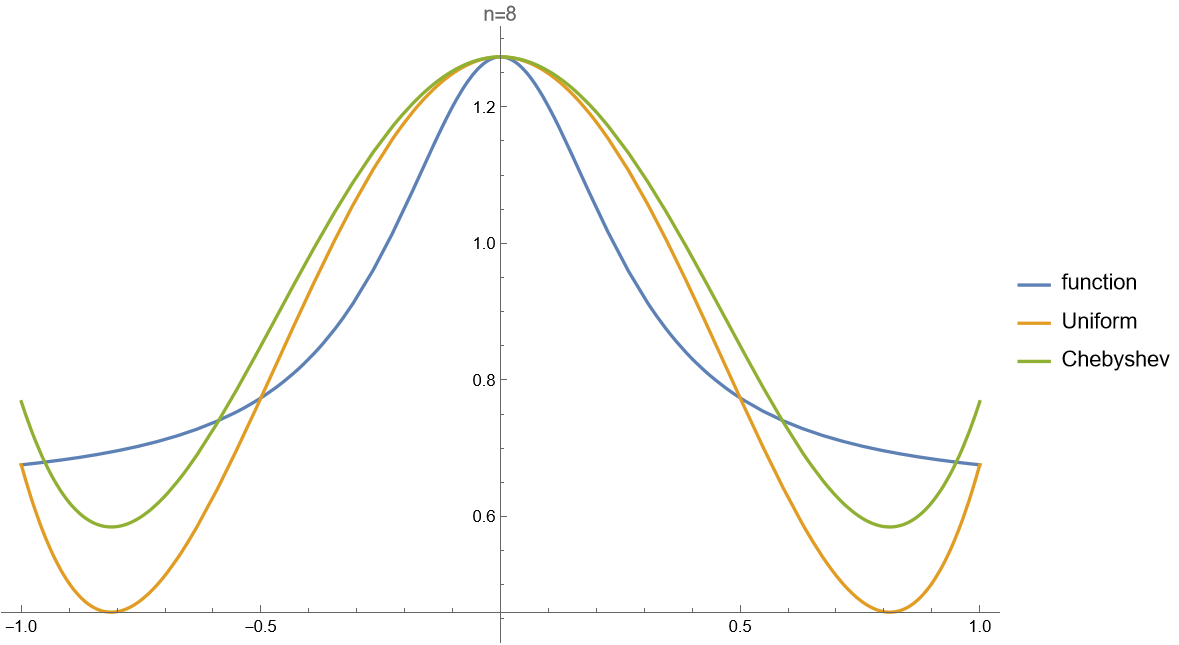
\includegraphics[width=\textwidth]{atan4.png}
        \caption{Интерполирование $y = \dfrac{1}{\arctg (1+10x^2)}$ для 4 узлов многочленом Лагранжа}
    \end{figure}
    \begin{figure}[H]
        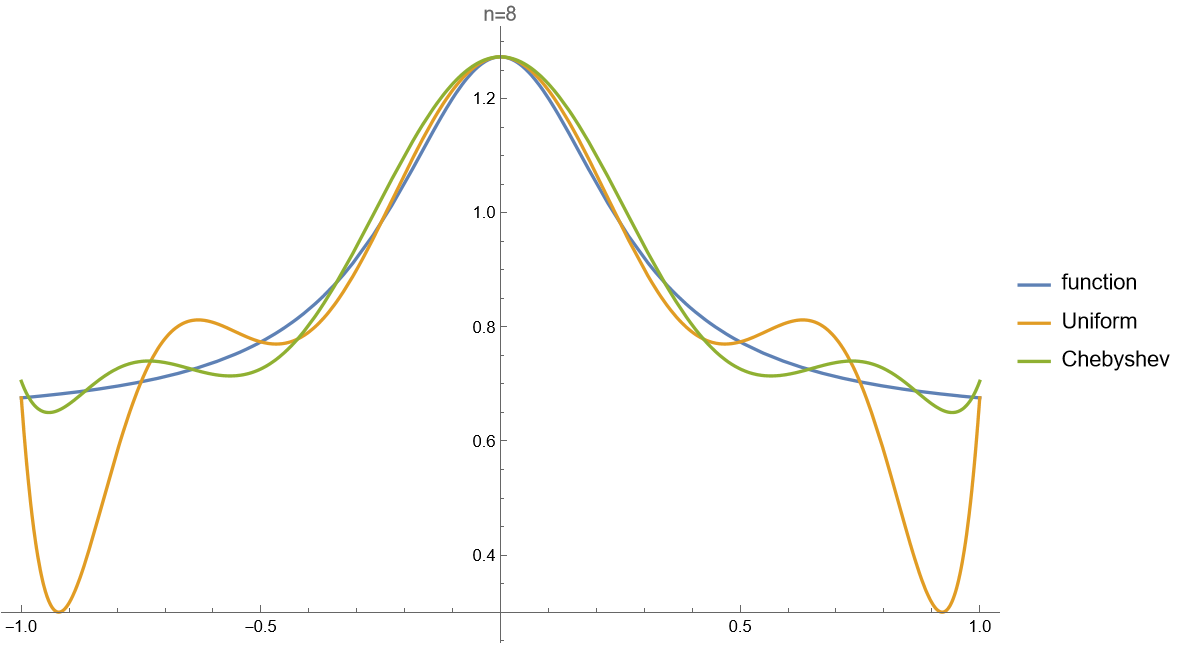
\includegraphics[width=\textwidth]{atan8.png}
        \caption{Интерполирование $y = \dfrac{1}{\arctg (1+10x^2)}$ для 8 узлов многочленом Лагранжа}
    \end{figure}
    \begin{figure}[H]
        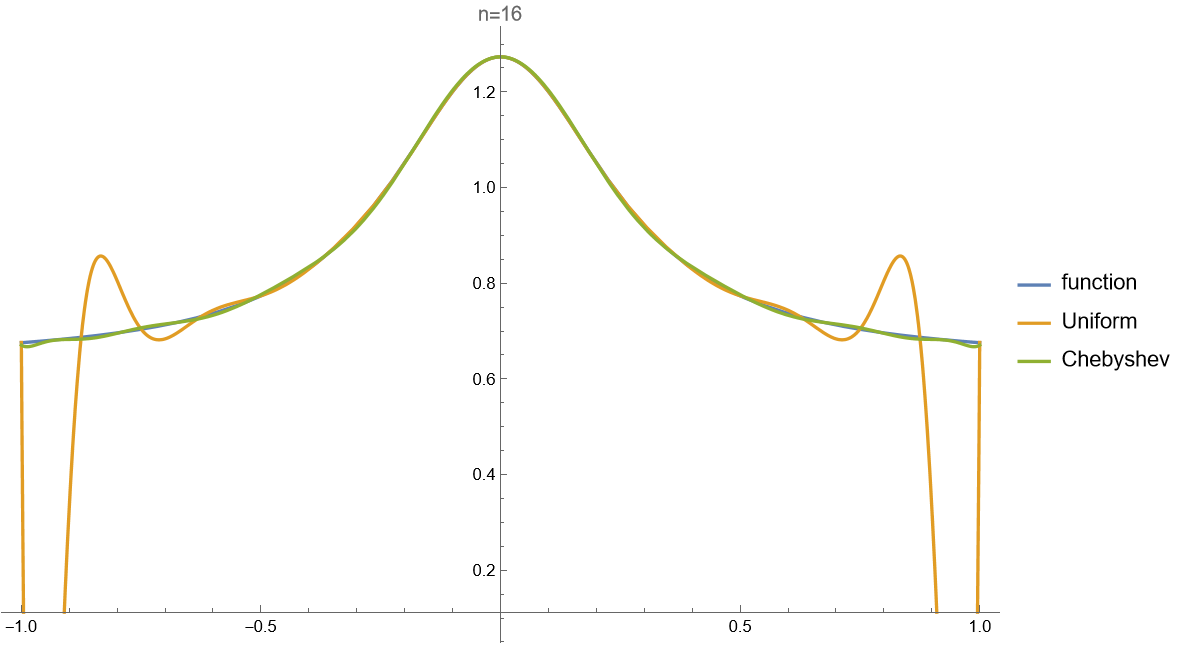
\includegraphics[width=\textwidth]{atan16.png}
        \caption{Интерполирование $y = \dfrac{1}{\arctg (1+10x^2)}$ для 16 узлов многочленом Лагранжа}
    \end{figure}
    \begin{figure}[H]
        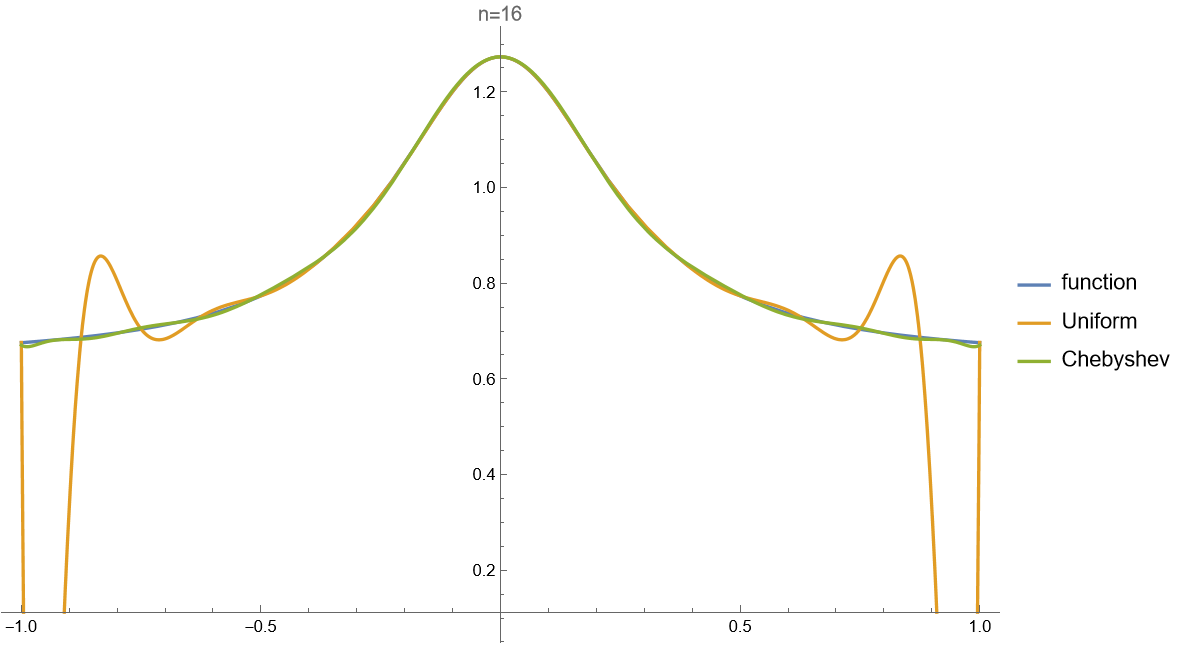
\includegraphics[width=\textwidth]{atan16.png}
        \caption{Интерполирование $y = \dfrac{1}{\arctg (1+10x^2)}$ для 16 узлов многочленом Лагранжа}
    \end{figure}
    \begin{figure}[H]
        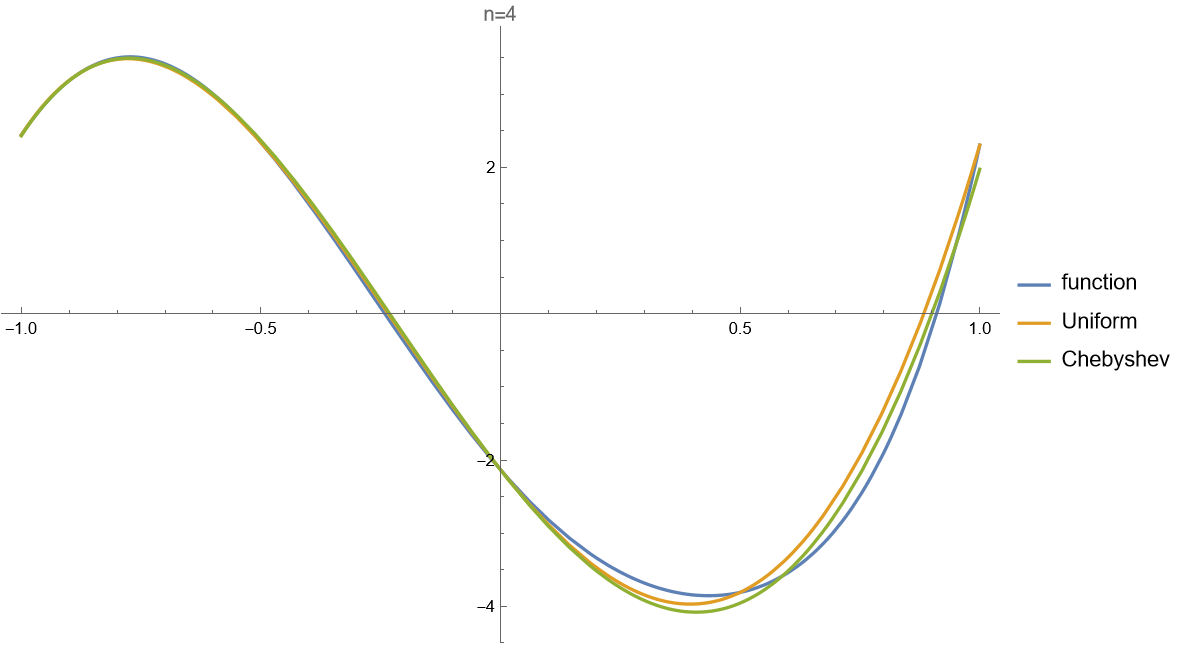
\includegraphics[width=\textwidth]{test4.png}
        \caption{Интерполирование $y = (4x^3 + 2x^2 - 4x + 2 )^{\sqrt{2}} + \arcsin{\dfrac{1}{5+x - x^2}} - 5$ для 4 узлов многочленом Лагранжа}
    \end{figure}
    \begin{figure}[H]
        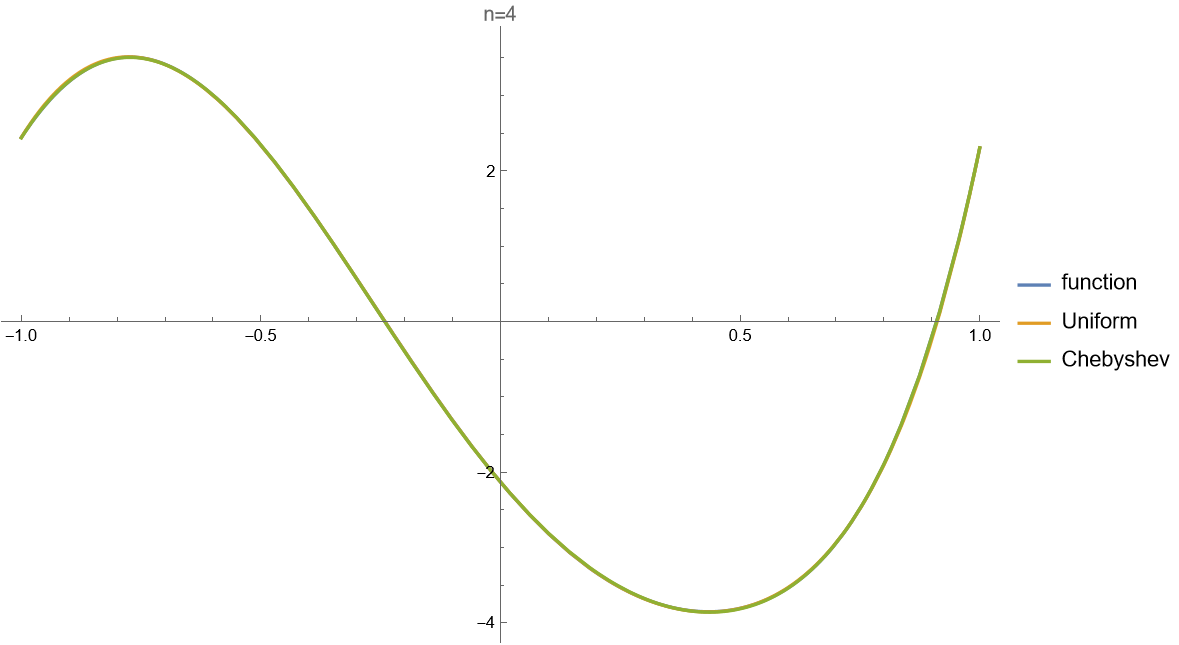
\includegraphics[width=\textwidth]{test8.png}
        \caption{Интерполирование$y = (4x^3 + 2x^2 - 4x + 2 )^{\sqrt{2}} + \arcsin{\dfrac{1}{5+x - x^2}} - 5$ для 8 узлов многочленом Лагранжа}
    \end{figure}
    \begin{figure}[H]
        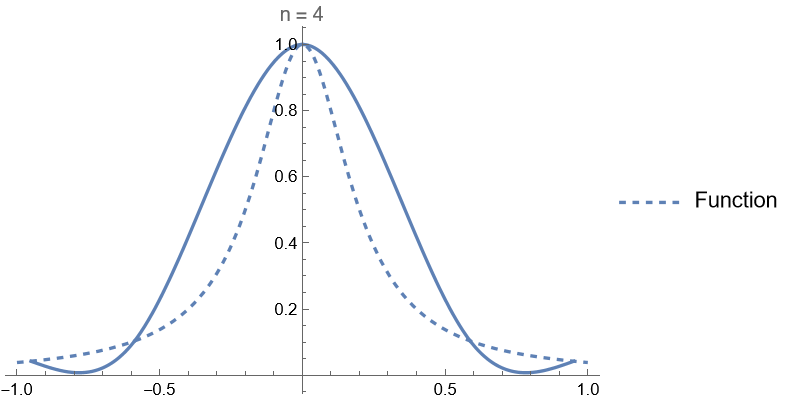
\includegraphics[width=\textwidth]{splinerunge4.png}
        \caption{{Интерполирование примера Рунге для 4 узлов сплайном}}
    \end{figure}
    \begin{figure}[H]
        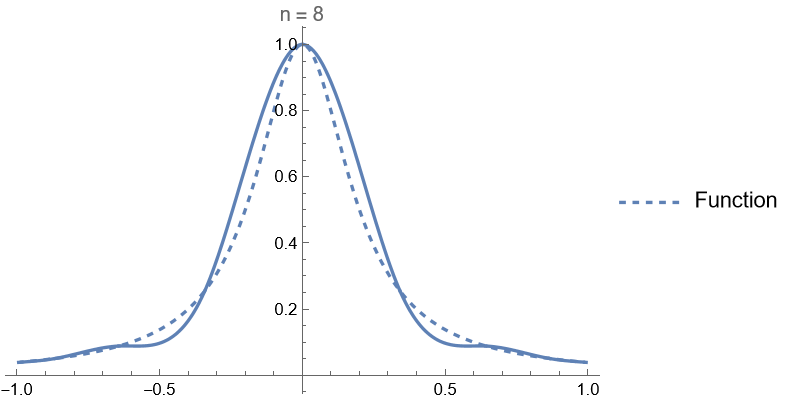
\includegraphics[width=\textwidth]{splinerunge8.png}
        \caption{{Интерполирование примера Рунге для 8 узлов сплайном}}
    \end{figure}
    \begin{figure}[H]
        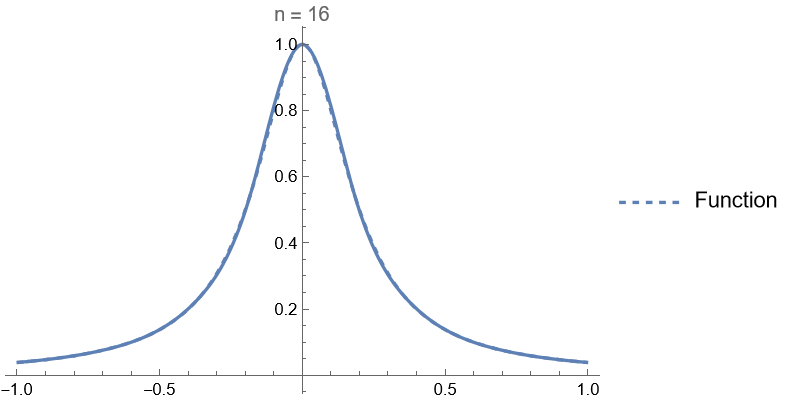
\includegraphics[width=\textwidth]{splinerunge16.png}
        \caption{{Интерполирование примера Рунге для 16 узлов сплайном}}
    \end{figure}
    \begin{figure}[H]
        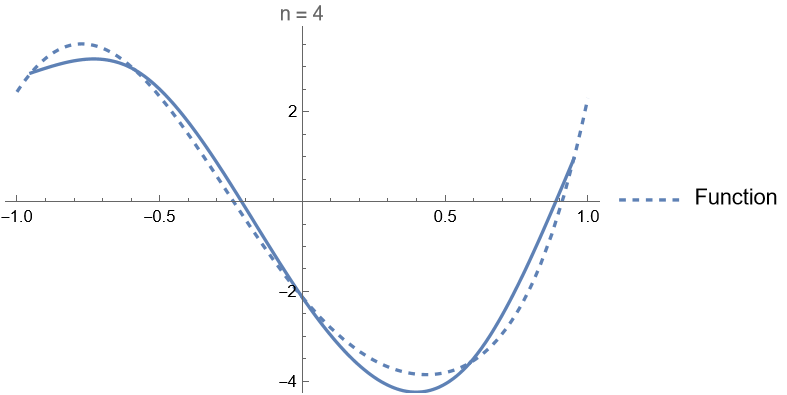
\includegraphics[width=\textwidth]{splinetest4.png}
        \caption{{Интерполирование $y = (4x^3 + 2x^2 - 4x + 2 )^{\sqrt{2}} + \arcsin{\dfrac{1}{5+x - x^2}} - 5$ для 4 узлов сплайном}}
    \end{figure}
    \begin{figure}[H]
        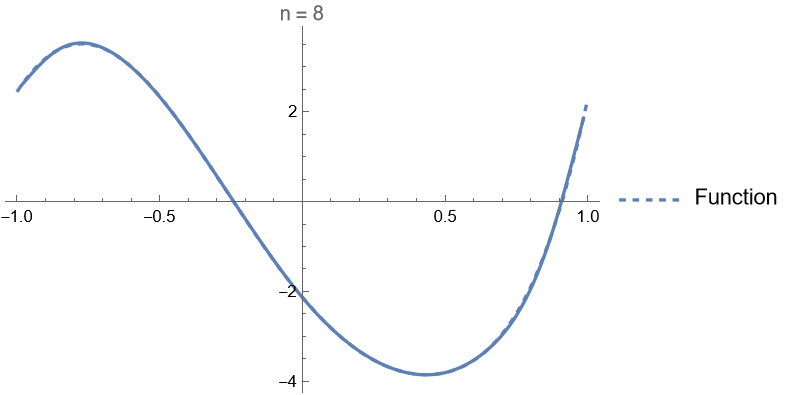
\includegraphics[width=\textwidth]{splinetest8.png}
        \caption{{Интерполирование $y = (4x^3 + 2x^2 - 4x + 2 )^{\sqrt{2}} + \arcsin{\dfrac{1}{5+x - x^2}} - 5$ для 8 узлов сплайном}}
    \end{figure}

=======
    
>>>>>>> 7cdee46c01cf605ac895434ec51f6a4b4065ba36
\end{document}
